% Include at a fixed width: scaling DOWN would push the
% in-figure type below the 9pt floor the artwork guide sets.
\begin{figure}[t]
  \centering
  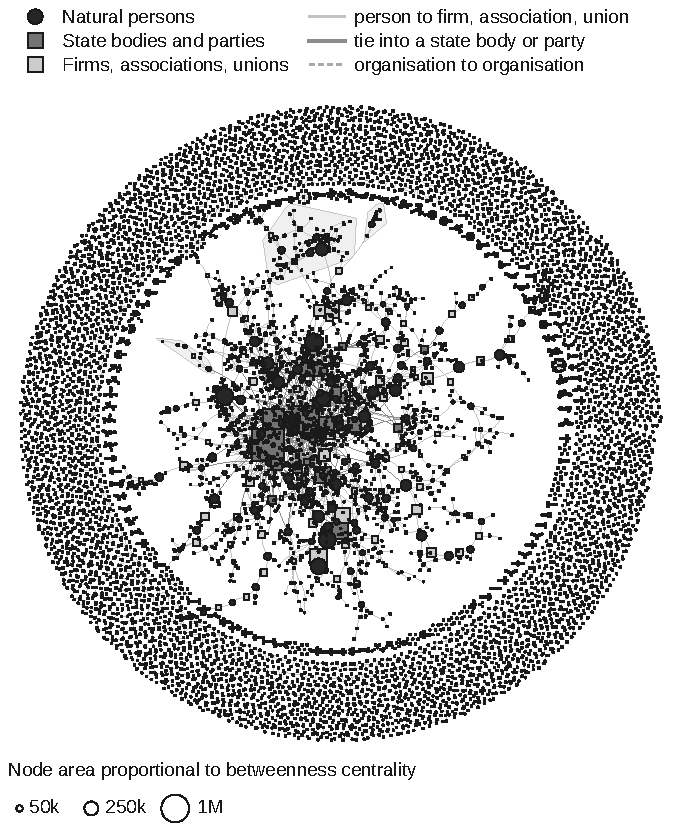
\includegraphics[width=4.5in]{fig16_brokerage_network_pre2011_all.pdf}
  \caption{\textbf{The Tunisian elite network before 2011-01-14.}
  Node area is proportional to betweenness centrality. Every entity and every tie is drawn
  and none is named: 9,734 entities joined by
  7,619 ties. The graph falls into 2,610 components,
  so the largest is laid out by force and the remaining 2,609
  fragments are packed into rings around it -- the positions of
  disconnected nodes are arbitrary, and a force layout spread these
  fragments over three quarters of the canvas, giving arbitrary structure
  the visual weight. Betweenness is exactly zero for 9,103 of them
  (94\%), which a strictly proportional area
  would render invisible, so area is proportional above a floor of
  0.9pt. Ties are those evidenced in the
  \emph{Journal Officiel} before 2011-01-14, the day Ben Ali left office:
  7,268 company board and officer ties and
  1,482 state offices, plus 119
  dated inter-organisational ties, over 9,734 entities in
  all. \textbf{This is a filter on source as well as on time.} Every
  gazette-evidenced tie in the dataset carries a date and every
  seed-derived tie carries none, so restricting to ties evidenced before a
  date necessarily drops the whole seed layer: shareholding, kinship,
  association and party membership are absent here, not because they did
  not exist before 2011, but because the roster that records them asserts
  present affiliations and is undated. Betweenness is recomputed on this
  graph and is not comparable with the pooled figure. The gazette also
  documents state appointments more completely than company officers,
  which will overstate the state's share relative to the private
  layer.
  The composition is 3,988 natural persons, 73 state bodies
  and parties, and 5,673 firms, associations and unions.}
  \label{fig:fig16_brokerage_network_pre2011_all}
\end{figure}

% ---------------------------------------------------------------------
% Accessibility description (APSR requires one; WCAG 2.1 AA)
% ---------------------------------------------------------------------
% A node-link diagram of 9734 entities connected by
% 7619 lines, drawn in greyscale. Circles are natural
% persons, squares are organisations; darker fills are state bodies and
% parties, lighter fills are firms, associations and unions. The area of
% each shape is proportional to its betweenness centrality, so the
% entities that lie on the most shortest paths appear largest. A small
% number of very large nodes sit at the centre of the diagram and connect
% several otherwise separate dense clusters of smaller nodes. No entity is
% named on the figure. A size key at the lower left gives
% reference areas in millions.
